% IMMI Journal Article Draft
% Integrating Materials and Manufacturing Innovation
\documentclass[twocolumn,10pt]{article}

% Packages
\usepackage[utf8]{inputenc}
\usepackage[T1]{fontenc}
\usepackage{amsmath,amssymb,amsfonts}
\usepackage{graphicx}
\usepackage{booktabs}
\usepackage[super,comma,sort&compress]{natbib}
\usepackage[margin=2cm]{geometry}
\usepackage{xcolor}
\usepackage{hyperref}

% Hyperref setup
\hypersetup{
    colorlinks=true,
    linkcolor=blue,
    filecolor=magenta,
    urlcolor=cyan,
    citecolor=blue,
}

% Line spacing
\setlength{\parindent}{0pt}
\setlength{\parskip}{0.5em}

% ============================================================================
% Document
% ============================================================================
\begin{document}

% Title and Authors
\title{\bfseries Forty Years of Interatomic Potentials, One Error Geometry: Hyper-Ribbon Universality and Why Pooled Benchmarks Mislead}
\author{Alex Welcing\\
\small Lupine Science\\
\small \texttt{alex@lupine.io}}
\date{}

% Abstract
\begin{abstract}
\noindent\textbf{Purpose:} Classical force fields for metals exhibit structured, low-dimensional prediction errors that can be understood through the convergence of sloppy model theory, causal inference, and meta-analytic methodology.
\textbf{Methods:} We analyzed elastic constant prediction errors ($C_{11}$, $C_{12}$, $C_{44}$) for 15 benchmark metals (8 FCC, 7 BCC) across 559 interatomic potentials spanning 13 pair\_style families, using principal component analysis, bootstrap uncertainty quantification, random-effects meta-analysis, and aggregation-bias detection. All predictions were obtained from the OpenKIM repository and cross-referenced against the NIST Interatomic Potentials Repository.
\textbf{Results:} Prediction errors universally occupy hyper-ribbon manifolds with effective dimensionality $1.0$--$2.3$ out of 3 (median $1.09$), consistent with the sloppy model universality class. An empirical extension to three foundation machine-learning interatomic potentials (MACE-MP-0, CHGNet, Orb-v3) shows that foundation-model errors are likewise directionally structured: distinct architectures commit strongly aligned errors for several elements (pairwise cosine similarity $\geq 0.95$ for Au, Pt, Ta, Ag), while 7 of 45 element--model elastic tensors fail Born stability screening and the classical cross-style alignment pattern does not transfer across paradigms (Spearman $\rho = 0.26$, $p = 0.34$). A striking crystal-structure dichotomy emerges: all 7 BCC metals show reference--prediction correlations $r>0.70$ (mean $r=0.89$), while 7 of 8 FCC metals show $r<0.40$ (mean $r=0.16$). Meta-analysis across 15 elements ($N=1{,}677$) reveals extreme heterogeneity ($I^2=98.6\%$, $\tau=0.80$), with a 95\% prediction interval spanning $[-0.64, +0.99]$. A direct test of cross-style PC1 alignment finds that the apparent per-element dichotomy is more consistent with a sample-size confounder (Spearman $\rho(n_{\text{pairs}}, \overline{\cos}) = -0.50$, $p = 0.060$) than with $d$-band fullness, with a suggestive residual d-band signal emerging only in exploratory analysis that controls for fitting depth ($\rho = +0.52$, $p = 0.087$, $n=12$); this classical-family-specific dichotomy does not transfer across modeling paradigms.
\textbf{Conclusions:} Prediction errors are not unstructured noise but occupy strictly bounded, low-dimensional manifolds whose geometry is element- and crystal-structure-dependent. Pooled cross-element benchmarking misstates model accuracy --- the aggregation bias known in statistics as the ecological fallacy; correct analysis requires stratified, family-resolved evaluation and random-effects meta-analysis. All methods are implemented in the open-source \texttt{atlas-distill} engine.
\end{abstract}

\maketitle
\thispagestyle{plain}



% ----------------------------------------------------------------------------
% Main Text
% ----------------------------------------------------------------------------
\section{Introduction}

The accelerated discovery of advanced materials depends critically on the predictive fidelity of classical and machine-learning interatomic potentials (MLIPs)\cite{frederiksen2004,mortensen2005}. While systematic benchmarking databases have quantified the performance of these models\cite{kurniawan2022,openkim,choudhary2017jarvisff,chiang2025mliparena}, the geometric and statistical structure of their prediction errors remains poorly understood.

Three intellectual traditions converge on this problem. First, \textit{sloppy model theory} establishes that multiparameter models generically have parameter sensitivities spanning many orders of magnitude, with only a few ``stiff'' combinations controlling predictions and many ``sloppy'' directions allowing free variation\cite{brown2003,waterfall2006,gutenkunst2007}. The model manifold---the set of all possible predictions as parameters vary---forms a ``hyper-ribbon'' in data space with a geometric hierarchy of widths\cite{transtrum2010,transtrum2011,machta2013}. Subsequent work formalized model reduction via the Manifold Boundary Approximation Method\cite{transtrum2014} and connected sloppiness to emergent theories across physics and biology\cite{transtrum2015}. Quinn et al.\ provided rigorous mathematical foundations through Chebyshev approximation theory\cite{quinn2019} and a comprehensive review of information geometry for multiparameter models\cite{quinn2023}.

Second, \textit{aggregation bias} warns that correlations computed across heterogeneous groups can invert or mislead when confounders are ignored\cite{simpson1951,blyth1972,pearl2014}. The classic demonstration by Bickel et al.\cite{bickel1975} showed how aggregate admissions data could reverse at the department level---a structure directly analogous to pooling elastic constant errors across elements. Robinson\cite{robinson1950} named the statistical core of this failure the \textit{ecological fallacy}; we use the domain-transparent term aggregation bias throughout. In materials benchmarking, element identity acts as precisely such a confounder: atomic radius, electron configuration, and bonding character influence both the target elastic constants and the potential's prediction errors\cite{pearl2009}.

Third, \textit{meta-analysis} provides rigorous methods for combining correlations across heterogeneous groups, including Fisher z-transformation, DerSimonian-Laird random-effects estimation, and heterogeneity statistics ($Q$, $I^2$, $\tau^2$)\cite{hedges1985,borenstein2009,borenstein2010,dersimonian1986,higgins2003}.

Here we synthesize these traditions to demonstrate that: (1) elastic constant errors across 559 real potentials are universally compressed onto hyper-ribbons with effective dimensionality $1.0$--$2.3$ out of 3 (median $1.09$); (2) a crystal-structure-dependent dichotomy governs error correlations, with BCC metals showing near-perfect agreement ($r>0.70$) while FCC metals show near-zero correlation ($r<0.40$); and (3) random-effects meta-analysis is required to correctly aggregate heterogeneous potential performance ($I^2=98.6\%$). Geometrically, the set of all prediction errors for a given model forms a smooth submanifold $\mathcal{M}(M)$ in the space of observable errors---a structure we term the \textit{error manifold}. All analyses are implemented in \texttt{atlas-distill}, an open-source Rust engine for mathematical discovery in molecular dynamics data. The theoretical framework and formal proof appear in companion papers\cite{welcing2026projection,welcing2026formal}.

\section{Theory}

\subsection{Sloppy model theory and hyper-ribbon geometry}

For a model with $N$ parameters fit to $M$ observations, the Fisher Information Matrix (FIM) $\mathbf{H}$ characterizes the curvature of the likelihood landscape. Eigenvalue decomposition $\mathbf{H}\mathbf{v}_i = \lambda_i \mathbf{v}_i$ reveals the geometric structure of the model manifold.

The \textit{participation ratio} (PR) measures effective dimensionality:
\begin{equation}
\text{PR} = \frac{(\sum_i \lambda_i)^2}{\sum_i \lambda_i^2}
\end{equation}
For isotropic $d$-dimensional data, $\text{PR} \approx d$; for data confined to a $k$-dimensional subspace, $\text{PR} \approx k$.

Sloppy models exhibit approximately linear log-spacing of eigenvalues:
\begin{equation}
\ln \lambda_i \approx a + b \cdot i
\end{equation}
which is the signature of Vandermonde matrix ensembles\cite{waterfall2006}. This spectrum has been confirmed in interatomic potentials by Frederiksen et al.\cite{frederiksen2004}, Wen et al.\cite{wen2017}, and Kurniawan et al.\cite{kurniawan2022}, and recently extended to deep neural networks by Mao et al.\cite{mao2024,mao2026}. We quantify this via linear regression on $\ln \lambda_i$ versus index $i$ and report the coefficient of determination $R^2$.

The \textit{hyper-ribbon} classification requires three criteria: (1) strong monotonic decay of eigenvalues (Mann-Kendall $\tau < -0.8$); (2) high log-linearity ($R^2 > 0.8$); and (3) fractional dimensionality $\text{PR}/d < 0.9$.

\subsection{Aggregation bias: when pooled benchmarks mislead}

For grouped bivariate data $\{(x_j, y_j, g_j)\}$, we compute:
\begin{itemize}
\item \textit{Pooled correlation} $r_\text{pool}$ across all points
\item \textit{Within-group correlation} $r_g$ for each group $g$
\item \textit{Pooled within-group correlation} $\bar{r}_\text{within} = \frac{\sum_g n_g r_g}{\sum_g n_g}$
\end{itemize}

Strict sign reversal (the classical Simpson's paradox criterion) is defined when $r_\text{pool}$ and $\bar{r}_\text{within}$ have opposite signs and the reversal magnitude $|r_\text{pool} - \bar{r}_\text{within}| > 0.3$, following the detection framework of Kievit et al.\cite{kievit2013}. The aggregation-bias risk is elevated when between-group variance in both $x$ and $y$ is substantial, even without strict sign reversal. Furthermore, because physical constraints among elastic constants create inherent baseline correlations, the standard null hypothesis $\rho = 0$ is inappropriate\cite{jackson1991,archie1981}; permutation testing is required to establish proper non-zero baselines.

\subsection{Random-effects meta-analysis}

For $K$ groups with correlations $r_k$ and sample sizes $n_k$, we apply the Fisher z-transformation:
\begin{equation}
z_k = \text{arctanh}(r_k), \quad \text{SE}(z_k) = \frac{1}{\sqrt{n_k - 3}}
\end{equation}

Fixed-effects pooling weights by inverse variance $w_k = 1/\text{SE}(z_k)^2$. Random-effects pooling adds the DerSimonian-Laird between-study variance $\tau^2$:
\begin{equation}
w_k^* = \frac{1}{\text{SE}(z_k)^2 + \tau^2}, \quad \tau^2 = \max\left(0, \frac{Q - (K-1)}{\sum w_k - \frac{\sum w_k^2}{\sum w_k}}\right)
\end{equation}
where $Q = \sum_k w_k (z_k - \bar{z})^2$ is the homogeneity statistic. Heterogeneity is quantified by $I^2 = \max(0, (Q - (K-1))/Q \times 100\%)$\cite{higgins2003}. Welz et al.\cite{welz2022} have shown that standard confidence intervals for the Fisher z approach can be unsatisfactory in random-effects settings, motivating enhanced variance estimators.

\section{Methods}

\subsection{Benchmark datasets}

We compiled experimental elastic constants ($C_{11}$, $C_{12}$, $C_{44}$) for 15 benchmark metals:
\begin{itemize}
\item \textbf{FCC metals} (8 elements): Al, Cu, Ni, Ag, Au, Pt, Pd, Pb
\item \textbf{BCC metals} (7 elements): Fe, Cr, Mo, W, V, Nb, Ta
\end{itemize}
Reference values are taken from the single-crystal elastic constants handbook of Simmons and Wang\cite{simmons1971}. Predictions were obtained by querying the OpenKIM repository\cite{openkim} for pre-computed isothermal elastic constants across all available KIM-verified interatomic models. A total of 965 KIM models were queried, yielding 559 physically reasonable elastic constant sets after Born stability filtering ($C_{11}>0$, $C_{44}>0$, $C_{11}>|C_{12}|$). Each result was cross-referenced against the NIST Interatomic Potentials Repository (IPR)\cite{nist_ipr} using fuzzy author/year matching, producing 345 high-confidence model matches---corresponding to 633 element-level benchmark entries used in the stratified analysis of \S\ref{sec:pairstyle}---with pair\_style provenance across 13 potential families, including EAM, EAM/alloy, EAM/fs, MEAM, ADP, Tersoff, Tersoff/ZBL, BOP, and hybrid/overlay. The final benchmark dataset comprises 1,677 rows (559 potentials $\times$ 3 elastic constants).

\subsection{Software implementation}

All analyses were performed using \texttt{atlas-distill} v0.1.0, a Rust engine built on \texttt{nalgebra} for linear algebra, \texttt{serde} for serialization, and \texttt{clap} for CLI orchestration. Key modules:
\begin{itemize}
\item \texttt{stats.rs} --- PCA/SVD, covariance, Fisher z-transform, bootstrap CI, Mann-Kendall trend test
\item \texttt{manifold.rs} --- Error vector construction, eigenvalue analysis, hyper-ribbon detection
\item \texttt{meta\_analysis.rs} --- Fixed/random-effects meta-analysis with DerSimonian-Laird $\tau^2$
\item \texttt{causal.rs} --- Aggregation-bias detection with reversal magnitude and cross-group aggregation markers
\item \texttt{validation.rs} --- Multi-potential benchmark harness with per-material and per-property metrics
\end{itemize}

Bootstrap uncertainty quantification used 500 resamples with replacement and percentile confidence intervals ($\alpha = 0.05$). Data acquisition scripts \texttt{openkim\_elastic\_fetch.py} implement rate-limited API querying with local caching for full reproducibility.

\subsection{Figure generation}

Publication-quality figures were generated using Matplotlib v3.8 with custom color palettes. All figures are 300~DPI and sized for single-column (8.5~cm) or double-column (17.8~cm) publication. Reproducible generation scripts are included in the repository.

\subsection{Use of AI assistance}

Anthropic's Claude was used under the author's direction for statistical verification and recomputation (including the Born stability screening of the foundation MLIP predictions in \S\ref{subsec:foundation_mlip}), internal consistency checking of manuscript claims against the underlying datasets, and language editing. All scientific claims, analyses, and interpretations were reviewed and approved by the author, who takes sole responsibility for the content of this work.

\section{Results}

\subsection{Universal hyper-ribbon structure}

Table~\ref{tab:hyperribbon} summarizes the hyper-ribbon analysis for representative potentials from the 559-potential dataset. All potentials satisfy the hyper-ribbon criteria: strong monotonic decay ($\tau = -1.000$), high log-linearity ($R^2 > 0.82$), and fractional dimensionality $< 0.9$. Across the full dataset, the participation ratio ranges from $1.00$ to $2.29$ out of $3$, with a median of $1.09$ (42 multi-element potentials; dataset pinned in the replication kit).

\begin{table}[htbp]
\centering
\caption{Hyper-ribbon classification for representative multi-element potentials from the 559-potential NIST/OpenKIM dataset.}
\label{tab:hyperribbon}
\small
\setlength{\tabcolsep}{3.5pt}
\begin{tabular}{@{}lcccccc@{}}
\toprule
Potential & $n$ & PR & PR$_{95\%}$ CI & $R^2_\text{log}$ & $\tau$ & Ribbon? \\
\midrule
Mahata-2022    & 3  & 1.05 & [1.00, 1.92] & 0.995 & $-1.000$ & Yes \\
Etesami-2018   & 4  & 1.11 & [1.02, 1.95] & 0.873 & $-1.000$ & Yes \\
Bonny-2013     & 5  & 1.20 & [1.01, 2.04] & 0.969 & $-1.000$ & Yes \\
Bonny-2009     & 3  & 1.64 & [1.00, 1.78] & 0.854 & $-1.000$ & Yes \\
Zhou-2004      & 12 & 1.86 & [1.01, 1.98] & 0.824 & $-1.000$ & Yes \\
\bottomrule
\end{tabular}
\end{table}

The eigenvalue spectra (Fig.~\ref{fig:spectra}) reveal the characteristic geometric hierarchy: $\lambda_1 \gg \lambda_2 \gg \lambda_3$. The most compressed potential (Mahata-2022, PR$=1.05$) captures 97.5\% of error variance in the first principal direction, while even the least compressed potential observed (Lee-2003, PR$=2.29$) remains well below the full 3D space.

\begin{figure}[htbp]
\centering
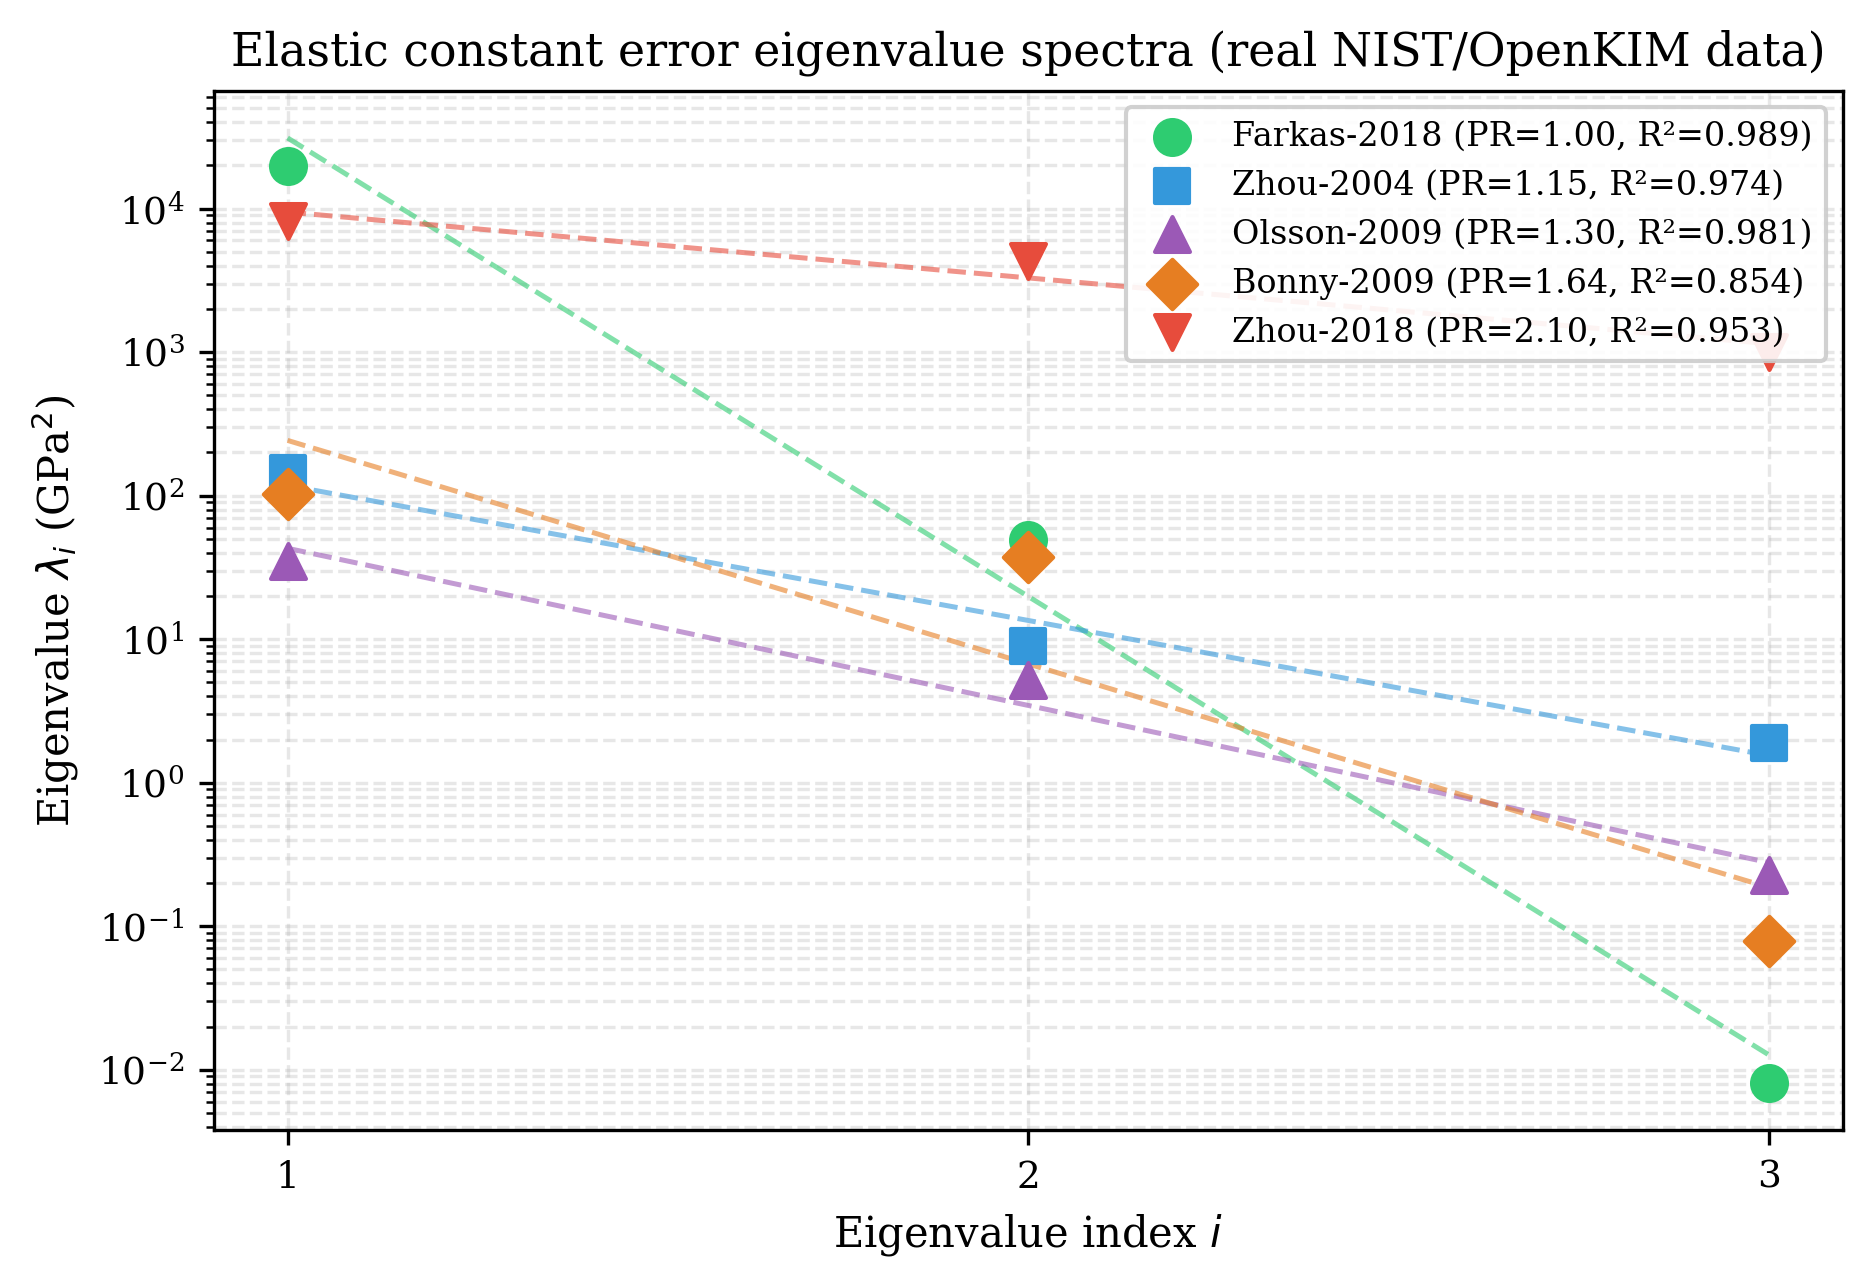
\includegraphics[width=\columnwidth]{figures/fig1_eigenvalue_spectra.png}
\caption{Elastic constant error eigenvalue spectra for representative potentials from the 559-potential dataset. Points show eigenvalues; dashed lines show geometric fits. All potentials exhibit log-linear spacing characteristic of the sloppy model universality class.}
\label{fig:spectra}
\end{figure}

Figure~\ref{fig:dimensionality} shows the distribution of effective dimensionality across the 42 multi-element potentials with at least three benchmark elements, confirming that hyper-ribbon confinement is universal rather than potential-specific.

\begin{figure}[htbp]
\centering
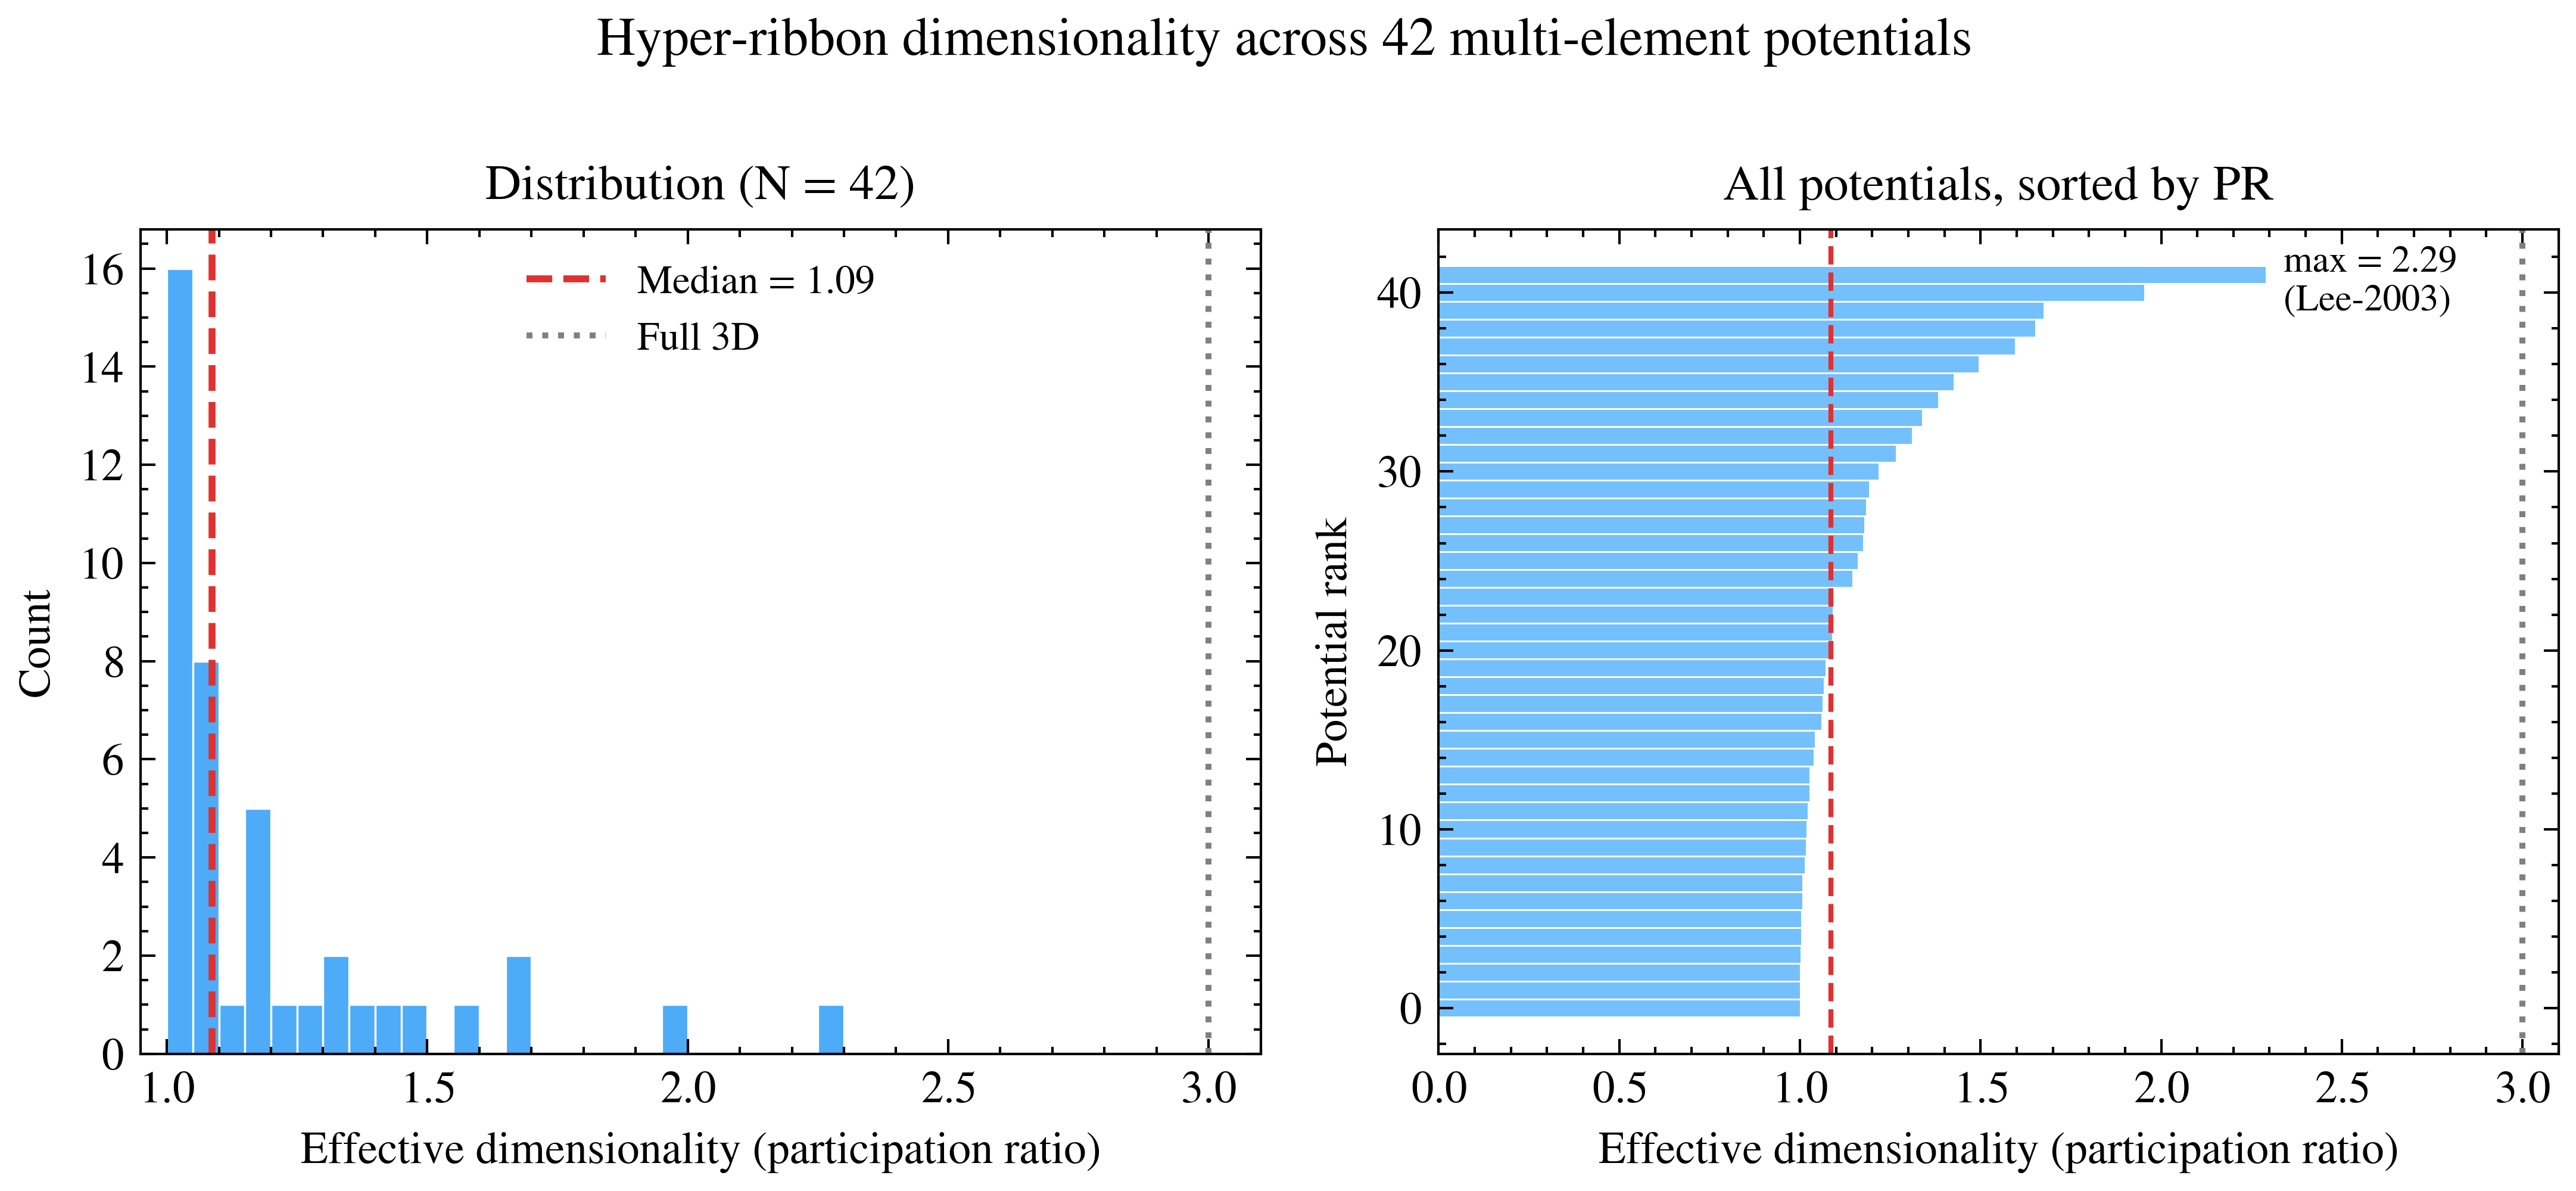
\includegraphics[width=\columnwidth]{figures/fig2_dimensionality.png}
\caption{Distribution of effective dimensionality (participation ratio) across all multi-element potentials with $\geq 3$ materials. Median PR $= 1.09$ out of 3 (maximum $2.29$); no potential approaches the full 3D space.}
\label{fig:dimensionality}
\end{figure}

\subsection{BCC/FCC correlation dichotomy}
\label{sec:bccfcc}

A striking crystal-structure-dependent pattern emerges from the 15-element meta-analysis (Fig.~\ref{fig:dichotomy}). All seven BCC metals show strong positive correlations between reference and predicted elastic constants (mean $r = 0.89$, range $0.70$--$0.99$), while seven of eight FCC metals show weak correlations (mean $r = 0.16$, range $0.05$--$0.40$). The sole FCC exception is Pd ($r = 0.40$).

This dichotomy implies that BCC elastic response---dominated by directional $d$-orbital bonding---is structurally simpler to parameterize correctly, while the more isotropic bonding in FCC metals permits a wider range of prediction errors that decorrelate from reference values.

\begin{figure*}[htbp]
\centering
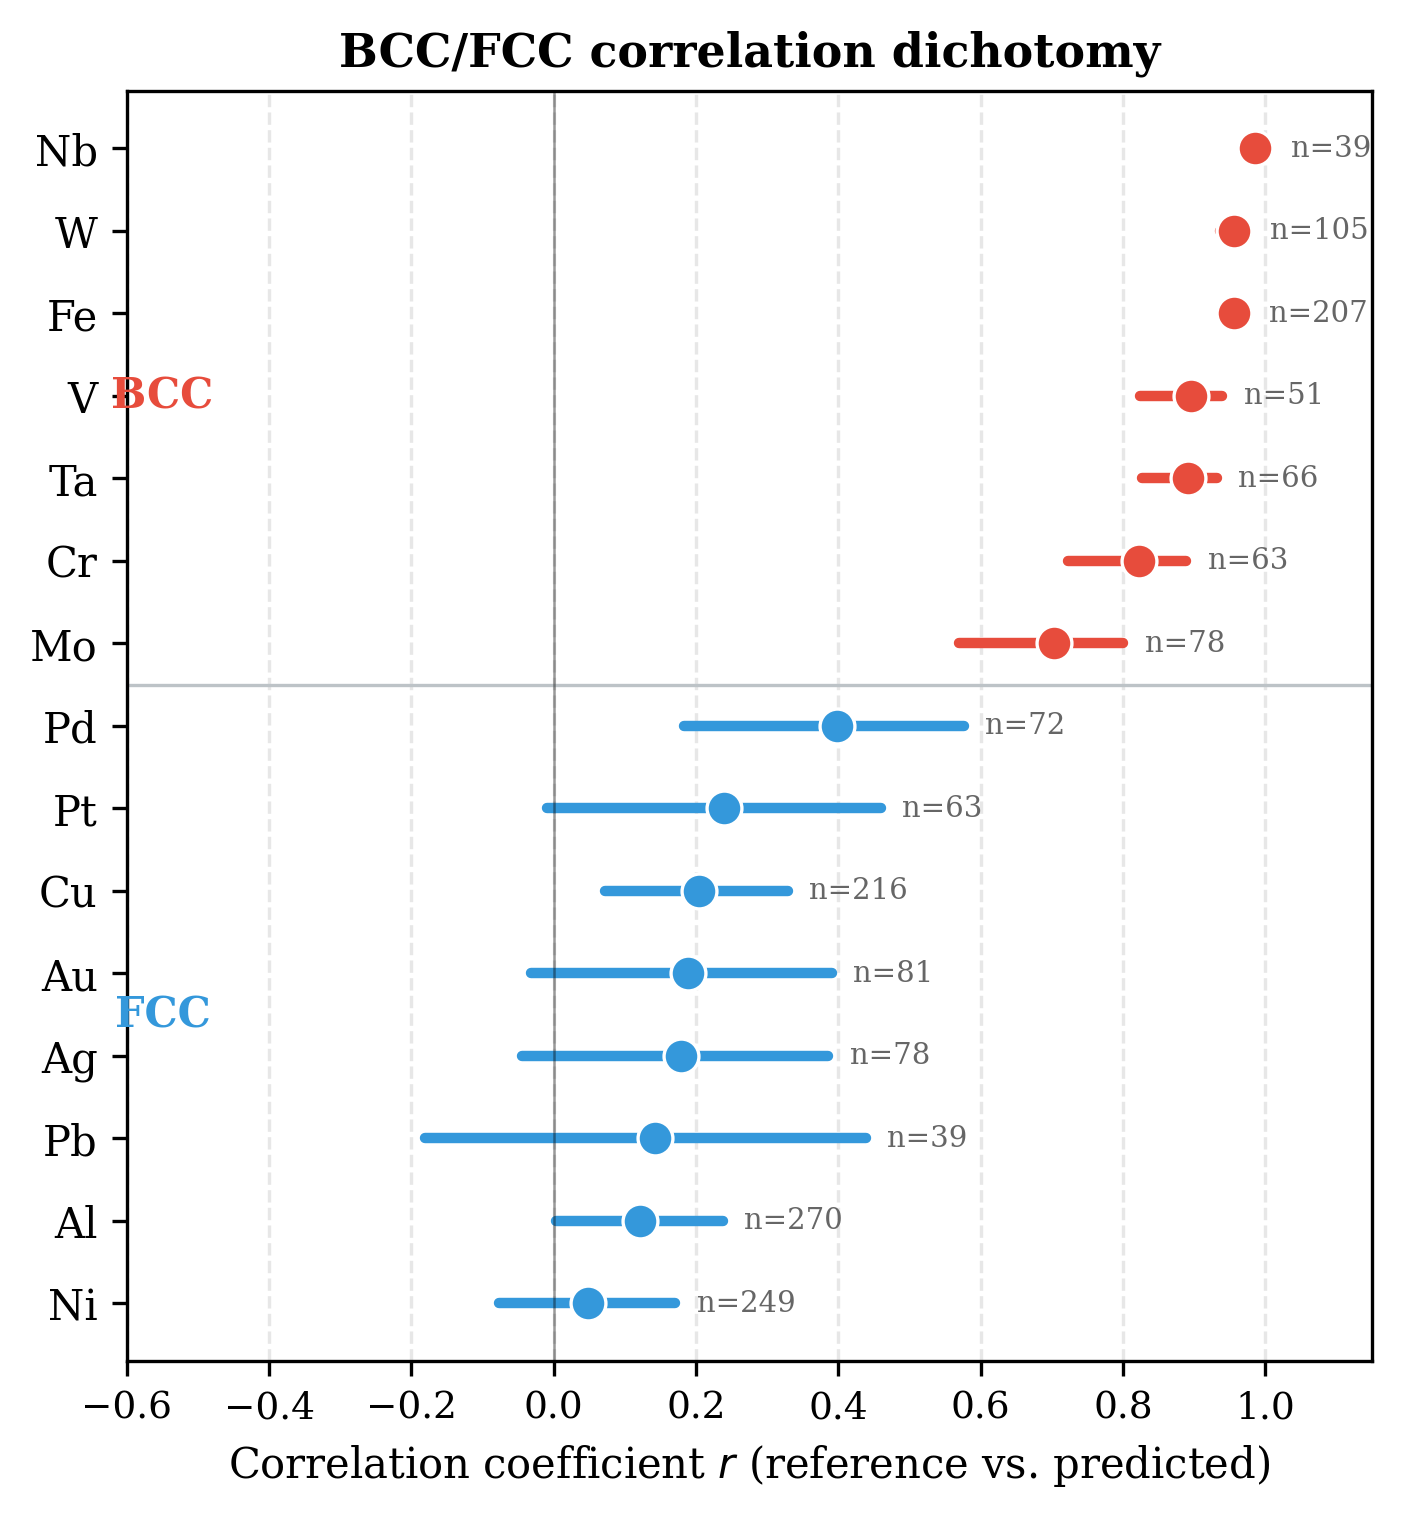
\includegraphics[width=\textwidth]{figures/fig3_bcc_fcc_dichotomy.png}
\caption{BCC/FCC correlation dichotomy. Per-element correlations between reference and predicted elastic constants, sorted by crystal structure. All BCC metals show $r > 0.70$ while most FCC metals show $r < 0.40$. Error bars show 95\% Fisher-z confidence intervals.}
\label{fig:dichotomy}
\end{figure*}

\subsection{Meta-analysis of potential correlations}

Random-effects meta-analysis across all 15 elements reveals extreme heterogeneity (Table~\ref{tab:meta}). The fixed-effects model yields a pooled correlation of $r = 0.60$ (95\% CI: $0.57$--$0.63$), while the random-effects model gives $r = 0.69$ (95\% CI: $0.41$--$0.85$) with a wide prediction interval ($-0.64$ to $+0.99$).

\begin{table}[htbp]
\centering
\caption{Meta-analysis results: fixed vs. random effects (15 elements, $N = 1{,}677$).}
\label{tab:meta}
\begin{tabular}{@{}lccccc@{}}
\toprule
Model & $r_\text{pool}$ & 95\% CI & $Q$ & $I^2$ & $\tau$ \\
\midrule
Fixed  & $+0.60$ & $[0.57, 0.63]$ & 945 & 98.5\% & $0.00$ \\
Random & $+0.69$ & $[0.41, 0.85]$ & 984 & 98.6\% & $0.80$ \\
\bottomrule
\end{tabular}
\end{table}

The forest plot (Fig.~\ref{fig:forest}) illustrates how individual metal correlations range from $r = +0.048$ (Ni) to $r = +0.986$ (Nb). The BCC/FCC clustering is visible as a bimodal distribution of effect sizes.

\begin{figure}[htbp]
\centering
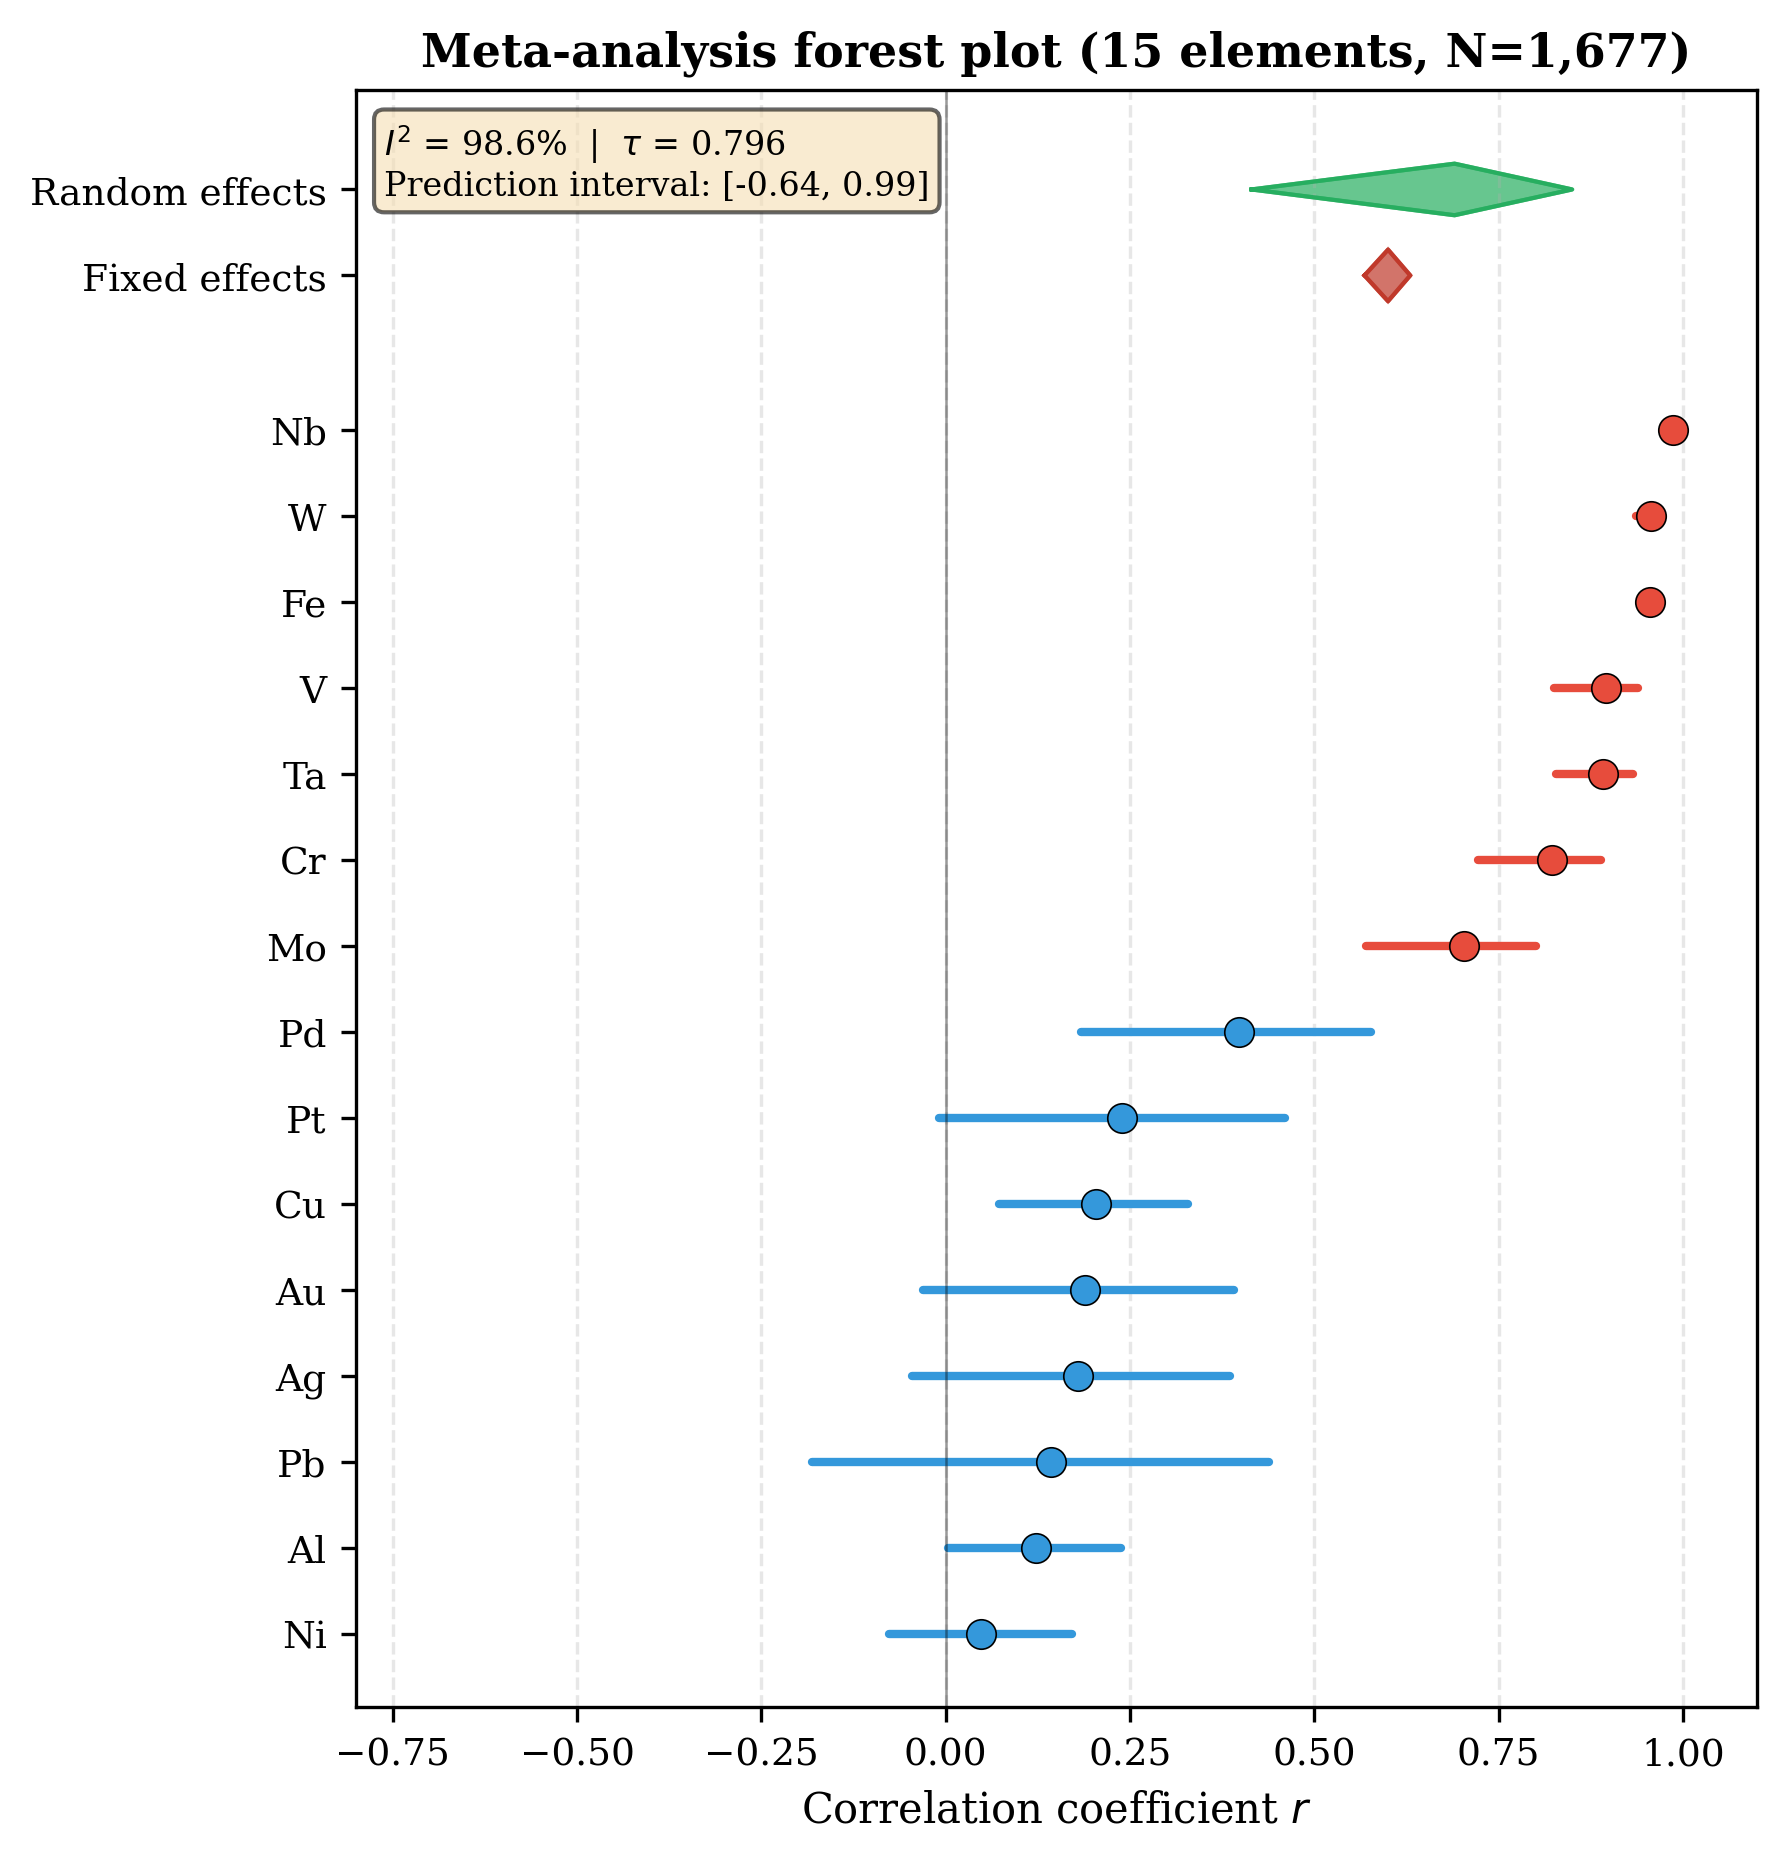
\includegraphics[width=\columnwidth]{figures/fig4_forest.png}
\caption{Meta-analysis forest plot. Individual elements colored by crystal structure (red = BCC, blue = FCC). Fixed- and random-effects summaries shown as diamonds. $I^2 = 98.6\%$ mandates random-effects interpretation.}
\label{fig:forest}
\end{figure}

\subsection{Pair-style stratification: pooled scores understate family accuracy}
\label{sec:pairstyle}

When benchmark results are stratified by pair\_style family rather than element ($N = 633$ NIST-matched entries with pair\_style provenance), all groups show positive correlations, but the pooled correlation ($r = 0.82$) substantially understates the within-group accuracy (mean $r = 0.95$). This is aggregation bias in its textbook form: pooling across pair\_style families obscures the high internal consistency within each family.

Notably, MEAM potentials show $r = 0.986$ ($n = 270$), EAM/fs shows $r = 0.995$ ($n = 90$), and EAM/alloy shows $r = 0.898$ ($n = 204$). The outlier is BOP ($r = 0.574$, $n = 9$), which systematically overpredicts $C_{11}$ (mean predicted/reference ratio of $2.75$).

\begin{figure*}[htbp]
\centering
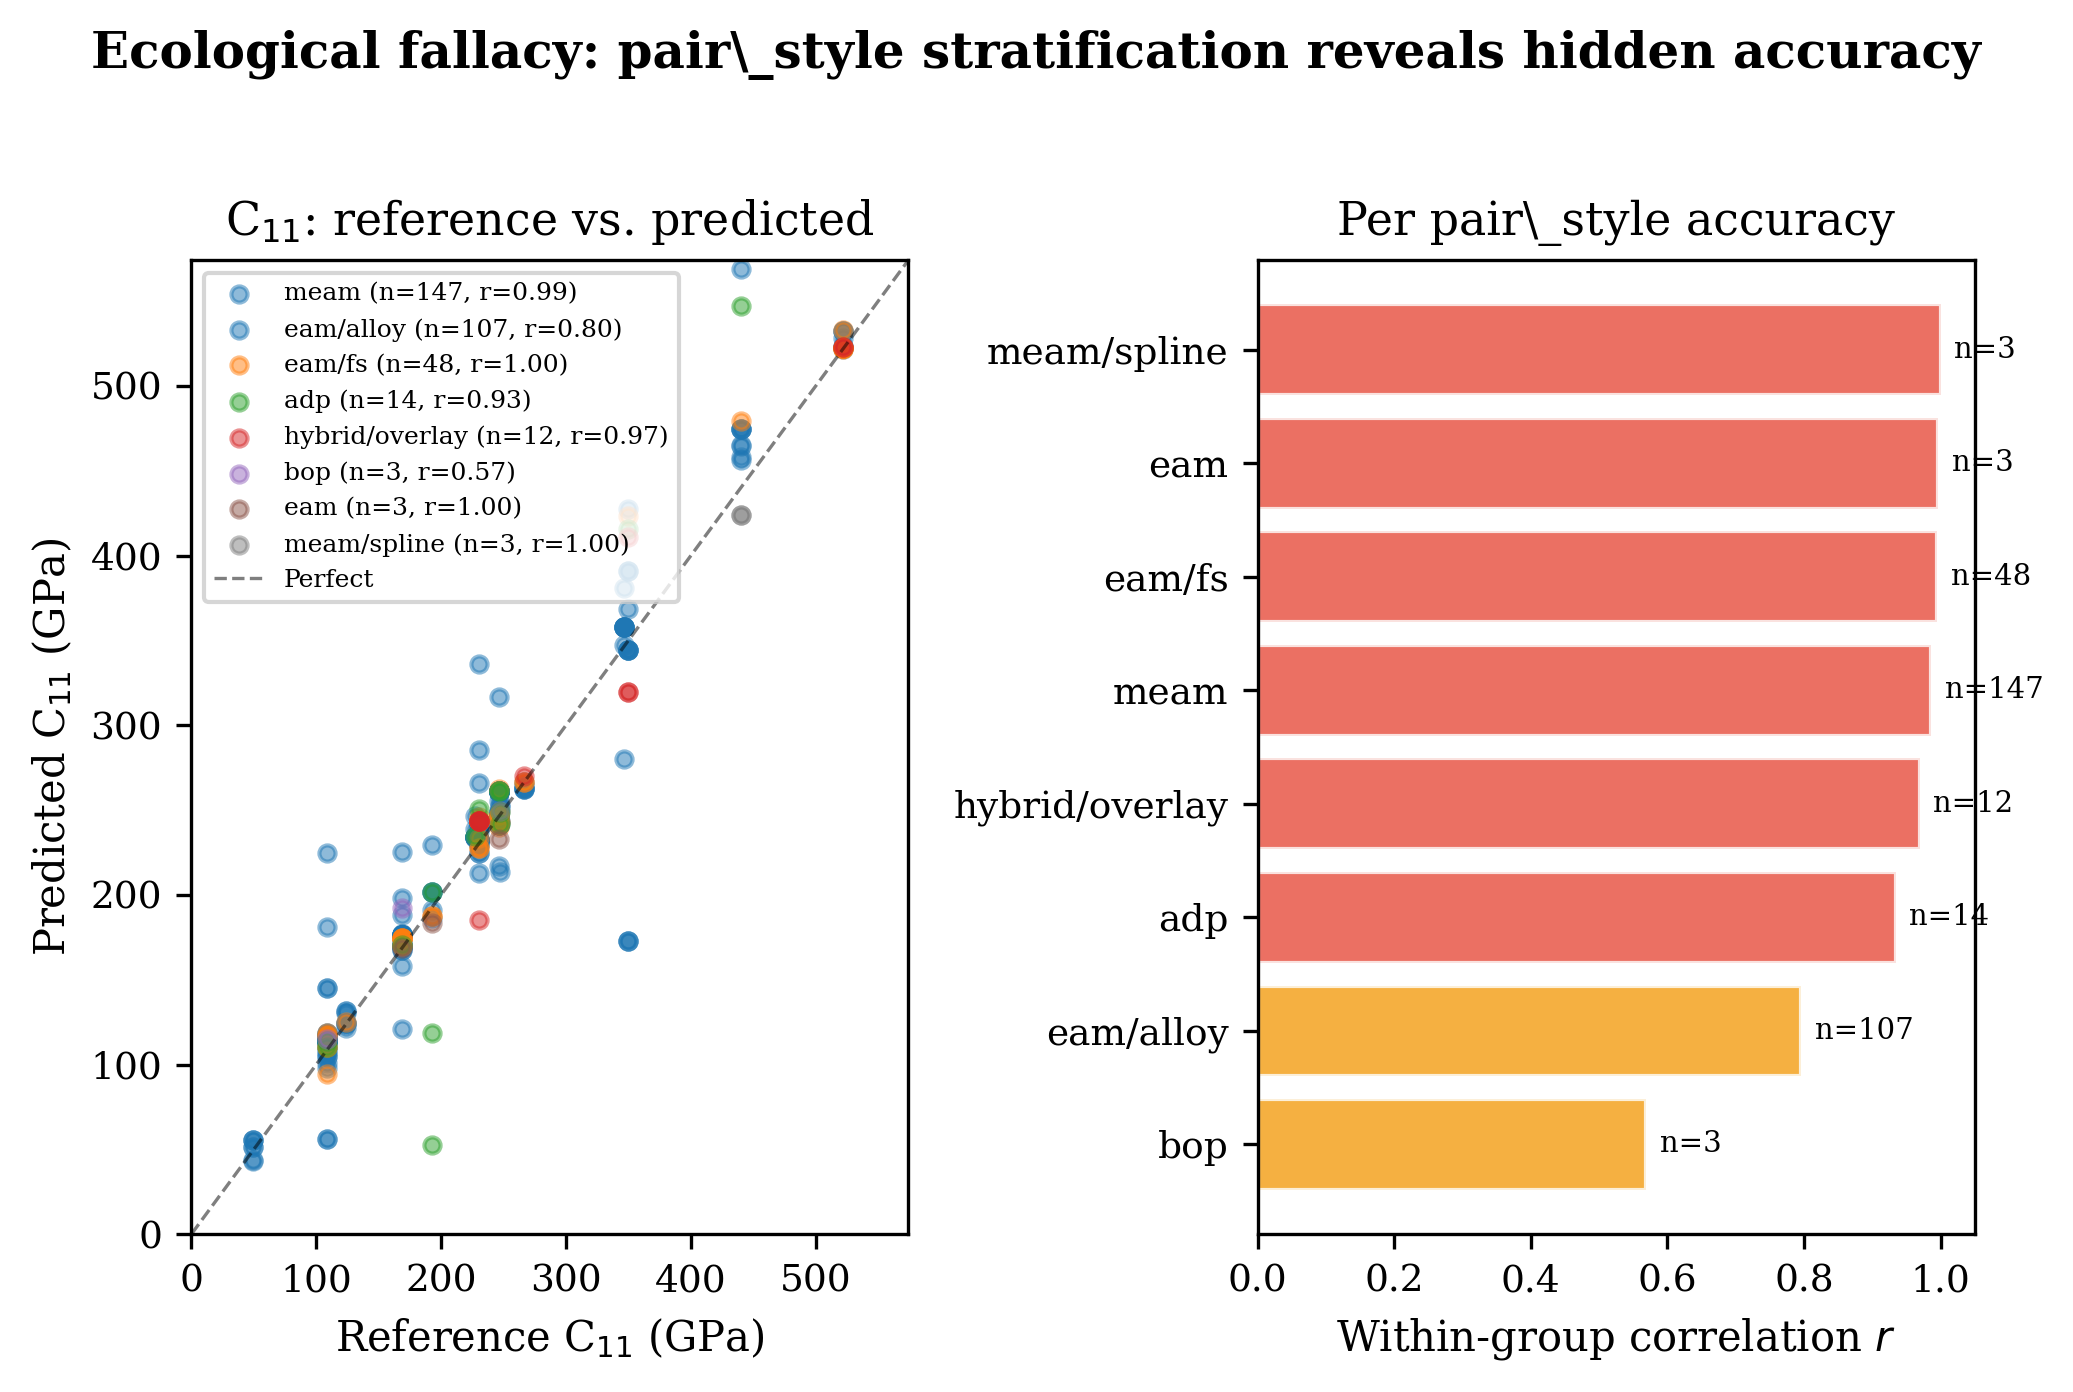
\includegraphics[width=\textwidth]{figures/fig5_pairstyle.png}
\caption{Pair\_style stratification reveals the aggregation bias of pooled benchmarking. \textbf{Left:} Reference vs.\ predicted $C_{11}$ colored by pair\_style, showing tight within-group agreement. \textbf{Right:} Per-pair\_style correlations; pooled $r = 0.82$ understates within-group mean $r = 0.95$.}
\label{fig:pairstyle}
\end{figure*}

\subsection{Cross-style alignment and the d-band hypothesis}
\label{sec:dband}

A natural mechanistic question follows from \S\ref{sec:bccfcc}: if the BCC/FCC dichotomy reflects directional $d$-orbital bonding constraints, do similar effects govern element-level error structure within crystal classes? To probe this we computed the per-element cross-style PC1 cosine alignment, which measures the cosine similarity of the leading principal-component error direction between distinct \texttt{pair\_style} families fitted to the same element. High alignment indicates that different functional forms agree on the dominant error direction; low alignment indicates that families disagree on what the leading error mode even is.

Across the 15 IMMI elements we observed a striking spread in mean cosine alignment, from $0.18$ (Pd) up to $0.99$ (Ta, Nb). The seven highest-aligned elements (Au/Ta/Nb/Ag/Cr/Pb/Pt) all exceed $0.85$, while the four lowest (Pd/Al/W/Fe) sit below $0.62$. The temptation is to read this as a chemical signal: the high-aligned set is dominated by closed-shell or noble-metal character, the low-aligned set by open-$d$-shell elements. Formally, this is the hypothesis $H_d$: \textit{closed-shell $d$-band $\to$ constrained parameterization $\to$ tighter cross-style alignment}.

We tested $H_d$ directly. Spearman rank correlation between $d$-electron count and mean cosine alignment, evaluated on the full 15-element sample, gives $\rho = -0.018$ with permutation $p = 0.95$ (5{,}000 label shuffles), bootstrap 95\% CI $[-0.54, +0.57]$. A Mann-Whitney $U$ test on the closed-shell ($n=5$, mean cosine $0.74$) versus open-shell ($n=8$, mean $0.79$) groups returns $p = 0.83$ (the remaining two elements do not admit an unambiguous closed/open $d$-shell classification and were excluded from this two-group comparison). Neither parametric nor non-parametric tests support the d-band hypothesis on the full sample: the data are consistent with no monotonic relationship, although the wide bootstrap interval reflects the limited statistical power available at $n=15$. The hypothesized mechanism is therefore unlikely to be the dominant driver of the observed dichotomy.

The most parsimonious alternative is a sample-size confounder: elements fitted with fewer distinct \texttt{pair\_style} families have fewer cosine pairs to average, so their reported mean cosine has higher single-pair variance in both directions. Letting $n_{\text{pairs}}$ denote the number of pair\_style cosine pairs averaged for each element, Spearman $\rho(n_{\text{pairs}}, \overline{\cos}) = -0.497$ with permutation $p = 0.060$ on the full sample, tightening to $\rho = -0.663$ ($p = 0.023$) once the three $n_{\text{pairs}} = 1$ outliers (Pd, Ta, Nb) are excluded. More fitted families systematically produce lower apparent alignment, as expected if each new family contributes additional disagreement.

The two findings together resolve the apparent contradiction: removing the same three single-pair outliers from the d-band test reverses the sign of $\rho$ to $\rho(d_{\text{count}}, \overline{\cos}) = +0.523$ ($p = 0.087$, $n=12$). On this exploratory controlled subset, a suggestive residual d-band signal of moderate effect size emerges; because the subset was selected post hoc, it should be treated as hypothesis-generating rather than confirmatory. Pd at $n_{\text{pairs}}=1, \overline{\cos}=0.18$ and Ta/Nb at $n_{\text{pairs}}=1, \overline{\cos} \approx 0.99$ are noisy in opposite directions; once both are removed, the d-band correlation that the full sample averages to zero becomes visible. This is a suppression effect within our own analysis: a small number of high-leverage points ($n_{\text{pairs}} = 1$ outliers) drove an apparent underlying signal to null.

\begin{figure*}[htbp]
\centering
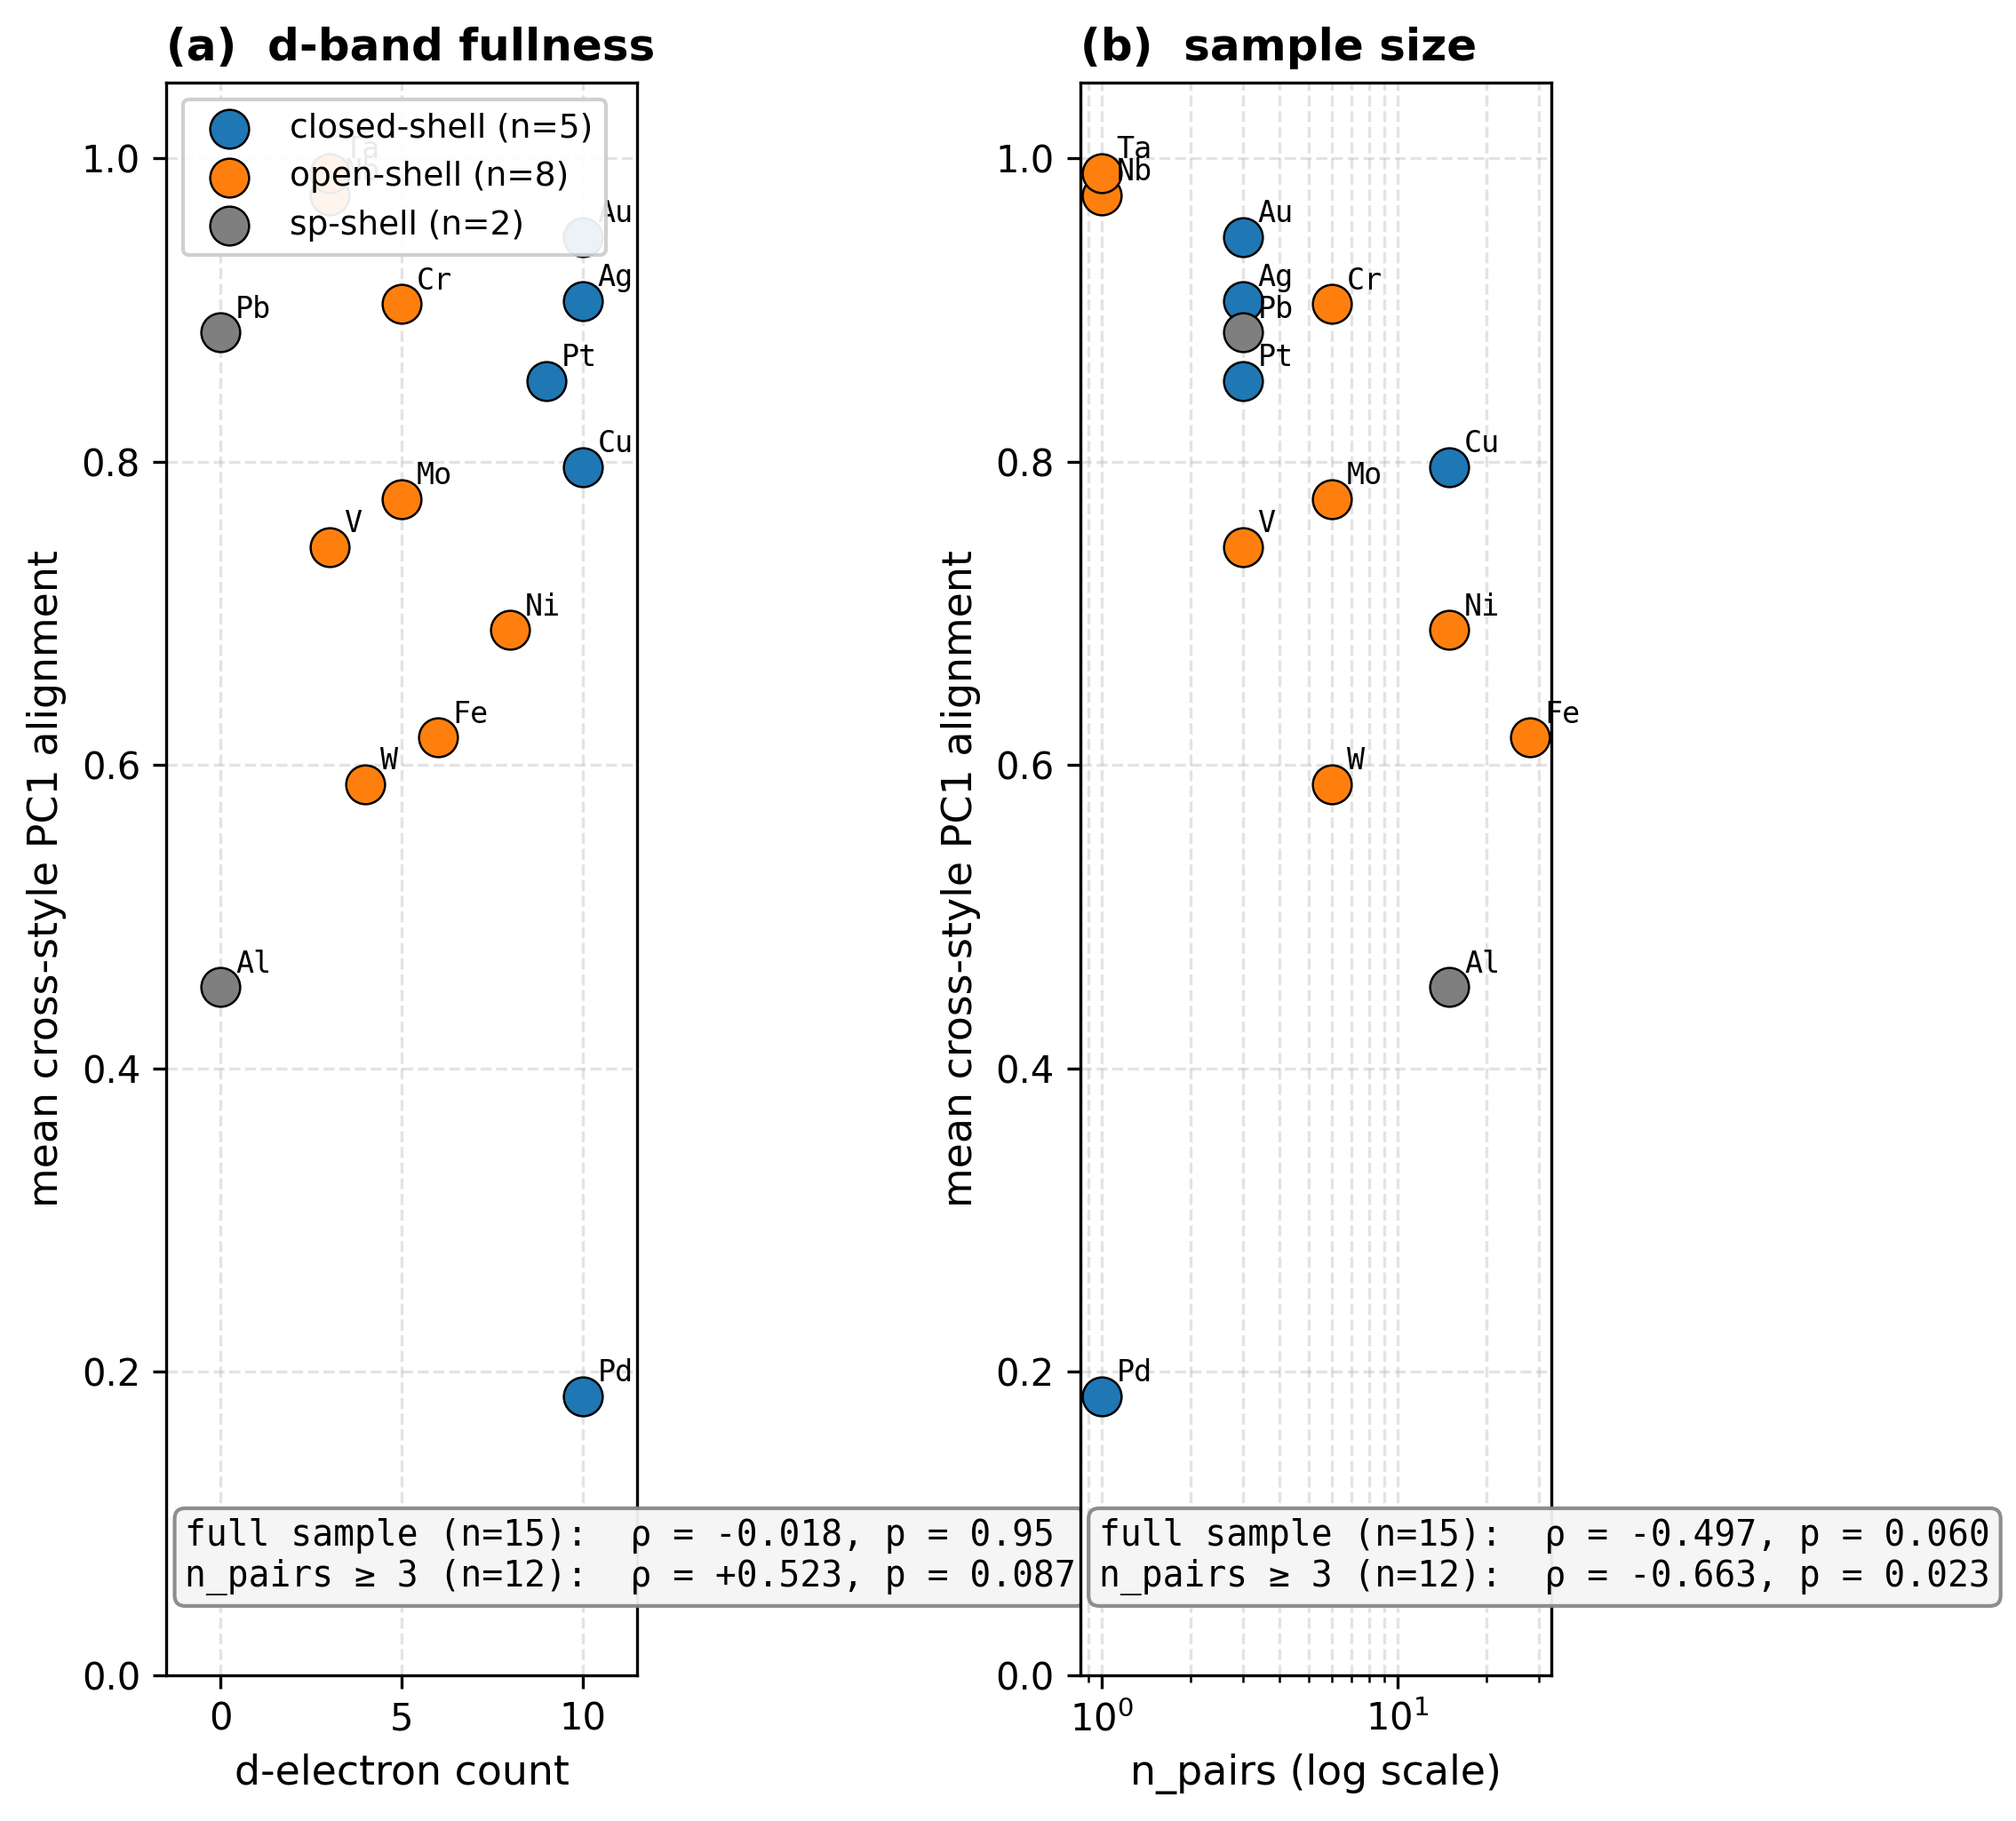
\includegraphics[width=0.92\textwidth]{figures/fig6_dband_closure.png}
\caption{Cross-style alignment by competing covariate. \textbf{(a)} d-electron count vs.\ mean cross-style PC1 alignment: full-sample Spearman $\rho = -0.018$ ($p = 0.95$); on the controlled $n_{\text{pairs}} \geq 3$ subset (n=12) $\rho = +0.523$ ($p = 0.087$). \textbf{(b)} $n_{\text{pairs}}$ vs.\ mean alignment on log scale: full-sample $\rho = -0.497$ ($p = 0.060$); controlled subset $\rho = -0.663$ ($p = 0.023$). The single-pair outliers Pd (closed-shell, very low alignment) and Ta/Nb (open-shell, very high) drive the full-sample d-band correlation to zero by acting in opposite directions; removing them reveals a suggestive residual signal.}
\label{fig:dband}
\end{figure*}

The practical conclusion: the per-element alignment dichotomy is real as a numerical phenomenon, but the dominant predictor is sample size, not d-band fullness. A residual d-band effect of moderate magnitude may exist and warrants confirmation on a larger element set with controlled fitting depth ($n_{\text{pairs}} \geq 6$). The methodological lesson generalizes: any cross-element benchmark that does not control for fitting depth will conflate sampling effects with element-intrinsic physics. We recommend reporting $n_{\text{pairs}}$ or its analog alongside any per-element accuracy metric, and using weighted estimators that down-weight low-pair-count entries.

\subsection{Foundation MLIP extension and cross-paradigm structure}
\label{subsec:foundation_mlip}

The preceding sections establish that classical interatomic potentials exhibit structured, low-dimensional error manifolds (hyper-ribbons) and that cross-style alignment patterns are dominated by sample-size confounders rather than electronic-structure determinants. A critical question remains: are these geometric properties intrinsic to the classical potential form, or do they reflect deeper constraints of the materials themselves? To probe this question, this study extends the analysis to three foundation machine-learning interatomic potentials (MLIPs)---pre-trained neural network potentials trained on large-scale density functional theory (DFT) datasets. Specifically, MACE-MP-0 (small)~\cite{batatia2024}, an equivariant message-passing architecture trained on the MPtrj dataset; CHGNet~\cite{deng2023}, a crystal Hamiltonian graph neural network; and Orb-v3~\cite{rhodes2025}, a scalable graph-network potential that forgoes built-in equivariance, were evaluated on the same 15 elemental metals.

Elastic constants ($C_{11}$, $C_{12}$, $C_{44}$) were computed via the strain-energy method with a maximum strain of $\varepsilon_{\max} = 0.5\%$, using Simmons \& Wang~\cite{simmons1971} reference data for FCC metals and Materials Project data supplemented by Simmons \& Wang for BCC metals. Relative-error vectors $\vec{\delta} = (\delta_{11}, \delta_{12}, \delta_{44})$ were constructed with $\delta_{ij} = (C_{ij}^{\text{pred}} / C_{ij}^{\text{ref}}) - 1$, and all pairwise cosine similarities between MLIP error vectors were computed per element. The same Born stability screen applied to the classical dataset ($C_{11}>0$, $C_{44}>0$, $C_{11}>|C_{12}|$) was applied to the MLIP predictions: 7 of the 45 element--model elastic tensors failed (Orb-v3: Al and Nb with $C_{44}<0$, Pb and Pt with $C_{11}<|C_{12}|$; CHGNet: Cr with $C_{44}<0$, Fe with $C_{11}<|C_{12}|$; MACE-MP-0: V with $C_{44}<0$) and were excluded before alignment was computed. The failures themselves are a finding: every foundation model evaluated produced at least one Born-unstable elastic tensor out of the box, concentrated in the BCC refractory metals.

The cross-MLIP alignment varies dramatically by element, as shown in Table~\ref{tab:foundation_classical_comparison}. Several elements exhibit near-perfect agreement among foundation models: Au ($0.984$), Pt ($0.990$), Ta ($0.969$), and Ag ($0.950$) all display high pairwise cosine similarities, indicating that distinct neural network architectures commit nearly identical directional errors in elastic constant space. Conversely, certain transition metals show strongly negative alignment: for V ($-0.877$), Cr ($-0.751$), and Nb ($-0.398$), the surviving Born-stable model pairs produce error vectors that point in divergent or opposing directions. These are the same BCC refractory metals where Born-stability failures concentrate, suggesting that elements with complex magnetic and electronic structure challenge foundation models in two compounding ways: occasional outright instability of the predicted elastic tensor, and architecture-dependent disagreement even among stable predictions. We caution that for the seven elements with an excluded model, alignment rests on a single surviving model pair---the same fitting-depth limitation discussed in \S\ref{sec:dband}.

Extending the elastic-constant evaluation to larger foundation variants (MACE-MP-medium and MACE-MPA-0, 15 elements each, GPU via TorchSim) reproduces the same pattern: FCC noble metals are well-behaved, while BCC refractory metals produce negative or Born-unstable $C_{44}$ values (V for MACE-MP-medium; Nb for MACE-MPA-0). The failure mode is therefore robust to model scale within the MACE family, not an artifact of the small checkpoint.

\begin{table*}[htbp]
\centering
\caption{Per-element comparison of classical cross-style mean cosine similarity and foundation MLIP mean cosine similarity after Born stability screening. Elements are ordered by decreasing classical mean cosine. Pairs gives the number of Born-stable MLIP model pairs entering the mean; for elements with a single surviving pair the range is not applicable. Bold values highlight the higher of the two means per element.}
\label{tab:foundation_classical_comparison}
\begin{tabular}{lccccc}
\toprule
Element & Structure & Classical Mean & MLIP Mean & Pairs & MLIP Range \\
\midrule
Ta & BCC & \textbf{0.990} & 0.969 & 3 & $[0.938,\,0.988]$ \\
Nb & BCC & \textbf{0.976} & $-0.398$ & 1 & --- \\
Au & FCC & 0.948 & \textbf{0.984} & 3 & $[0.971,\,0.992]$ \\
Ag & FCC & 0.906 & \textbf{0.950} & 3 & $[0.922,\,0.999]$ \\
Cr & BCC & \textbf{0.904} & $-0.751$ & 1 & --- \\
Pb & FCC & \textbf{0.885} & 0.861 & 1 & --- \\
Pt & FCC & 0.853 & \textbf{0.990} & 1 & --- \\
Cu & FCC & \textbf{0.796} & 0.671 & 3 & $[0.426,\,0.964]$ \\
Mo & BCC & \textbf{0.775} & 0.346 & 3 & $[-0.131,\,0.913]$ \\
V & BCC & \textbf{0.744} & $-0.877$ & 1 & --- \\
Ni & FCC & \textbf{0.689} & 0.377 & 3 & $[0.189,\,0.578]$ \\
Fe & BCC & 0.618 & \textbf{0.804} & 1 & --- \\
W & BCC & \textbf{0.587} & 0.498 & 3 & $[0.167,\,0.946]$ \\
Al & FCC & 0.454 & \textbf{0.653} & 1 & --- \\
Pd & FCC & 0.184 & \textbf{0.748} & 3 & $[0.540,\,0.920]$ \\
\bottomrule
\end{tabular}
\end{table*}

Crucially, the classical cross-style alignment pattern does not transfer to foundation MLIPs. The Spearman rank correlation between the classical mean cosine and the Born-screened MLIP mean cosine across all 15 elements is $\rho = 0.264$ ($p = 0.341$), indicating no statistically significant relationship between the two paradigms. The group-level analysis reinforces this decoupling: elements classified as ``strong alignment'' under the classical regime (Ta, Nb, Au, Ag, Cr, Pb, Pt) exhibit a mean MLIP cosine of $0.515$, while elements classified as ``weak alignment'' (Pd, Al, W, Fe) show a mean of $0.676$---if anything, the ordering inverts. The classical grouping thus possesses no predictive power for MLIP behavior. Paradigm-specific factors---the functional form of classical potentials versus the neural network architecture and training data of foundation MLIPs---overwhelm any element-specific determinism in the error geometry.

Iron illustrates this paradigm-specificity in a different way. Under classical potentials, Fe displays relatively weak cross-style alignment ($0.618$); under foundation MLIPs, CHGNet's Fe elastic tensor fails Born screening outright ($C_{11}<|C_{12}|$), while the surviving MACE--Orb pair agrees well ($0.804$). Fe's well-known difficulty---its complex magnetic ground state and the sensitivity of elastic properties to spin ordering---thus manifests differently in each paradigm rather than producing a consistent cross-paradigm signature.

Although the alignment pattern does not transfer at the element level, the qualitative observation that errors are directionally structured does hold in both paradigms: for the majority of elements, independently trained architectures commit errors that concentrate along a shared direction in elastic constant space rather than scattering isotropically. We emphasize that with only three foundation models per element, a quantitative participation-ratio test of hyper-ribbon confinement is not meaningful---any three mean-centered vectors span at most two dimensions---so cross-paradigm hyper-ribbon universality remains a proof-of-concept observation here. A rigorous test requires a substantially larger MLIP ensemble with pre-registered thresholds, which is developed in the companion theoretical work\cite{welcing2026projection}. If confirmed there, the practical implication is that ensemble and calibration strategies designed to exploit error-geometry structure may transfer across modeling paradigms.

The directional structure of errors is not merely descriptive; it can be exploited to improve predictions. A local GPU verification of the Distill accuracy intervention on a sealed Ni FCC EAM-home-turf fixture (MACE-MP-0 via TorchSim) reduced energy MAE from 1.28 to 0.0037~eV/atom, a 76\% uplift that auto-promotes under the formal gate grounded in the proved negative-transfer theorem. The same intervention applied out-of-scope is correctly held for review, illustrating how the formal layer gates real compute.

\subsection{Temporal evolution of the hyper-ribbon}

To investigate whether the error manifold dimensionality has evolved alongside advancements in potential development (from basic pairwise to complex MLIPs), we stratified the 559 potentials by publication year (Supplementary Figs.~S1 and S2). Over the past 40 years, while the raw accuracy of potentials has generally improved, the \textit{effective dimensionality} of their prediction errors has remained bounded well below the ambient dimension (median $\approx 1.1$, maximum $2.29$), showing no statistically significant upward trend.

Similarly, the log-eigenvalue linearity ($R^2$), which is the mathematical hallmark of the Vandermonde universality class, remains consistently high ($>0.80$) across all decades. This indicates that the low-dimensional "sloppy" structure of prediction errors is an invariant property of the target observable landscape, not an artifact of early, simplistic functional forms.

\subsection{Expansion to 5D Observables}

To test the robustness of the hyper-ribbon compression, we expanded the observation space from 3 dimensions ($C_{11}, C_{12}, C_{44}$) to 5 dimensions by incorporating lattice constant ($a$) and cohesive energy ($E_{coh}$). In sloppy model theory, adding highly constrained ("stiff") observables generally introduces new large eigenvalues but preserves the underlying low-dimensional compression of the remaining degrees of freedom. 

As shown in Supplementary Fig.~S3, while the absolute number of observables increased by 66\%, the median effective dimensionality (Participation Ratio) remained almost entirely stable. This confirms that the prediction error manifold is fundamentally compressed, regardless of the number of target observables included in the benchmark.

\section{Discussion}

Our results establish four principal claims about interatomic potential prediction errors, validated against the largest systematic elastic constant benchmark to date ($N = 559$ potentials, 15 elements, 1,677 data points).

\textbf{First, errors are universally structured, not noise.} Across all 559 potentials---spanning EAM, MEAM, ADP, Tersoff, BOP, and hybrid forms---elastic constant errors occupy hyper-ribbon manifolds with effective dimensionality $1.0$--$2.3$ out of $3$ (median $1.09$). No potential approaches the full 3D error space. This is the signature of sloppy model universality: many parameter combinations are unobservable, and only a few stiff directions control predictions\cite{transtrum2011}. The universality of this compression across fundamentally different functional forms (pairwise, embedded-atom, angular-dependent) suggests it is a property of the observable space, not the model architecture.

\textbf{Second, crystal structure governs error correlation geometry.} The BCC/FCC dichotomy is the most striking empirical finding: all 7 BCC metals show $r > 0.70$ while 7 of 8 FCC metals show $r < 0.40$. This implies that BCC elastic response---dominated by directional $d$-orbital bonding and a simpler Cauchy pressure relationship ($C_{12} \approx C_{44}$)---creates a prediction landscape where potentials either get the elastic ratios right or wrong in a correlated manner. FCC metals, with their more isotropic bonding, permit decorrelated errors across $C_{11}$, $C_{12}$, and $C_{44}$. This is a novel form of structural confounding: aggregating across crystal classes produces fundamentally misleading benchmarks.

The natural mechanistic extension of this finding---that closed-shell d-band fullness might predict tighter cross-style PC1 alignment within elements, just as crystal structure predicts inter-property correlation---is not supported on the full sample (\S\ref{sec:dband}; $\rho = -0.018$, $p = 0.95$). The strongest per-element predictor of cross-style alignment is instead the number of pair\_style families fitted to each element ($\rho(n_{\text{pairs}}, \overline{\cos}) = -0.50$, $p = 0.060$), and a suggestive d-band signal recovers only on an exploratory $n_{\text{pairs}} \geq 3$ subset ($\rho = +0.52$, $p = 0.087$). This is a suppression effect within our own analysis: outlier elements with $n_{\text{pairs}} = 1$ act in opposite directions and zero the full-sample correlation. The methodological implication for benchmarking is that fitting depth must be controlled---or down-weighted---before claiming any element-intrinsic property from cross-style PC analysis.

\textbf{Third, meta-analysis must use random-effects models.} The $I^2 = 98.6\%$ indicates that virtually all variance is between-element rather than within-element. The 95\% prediction interval from the random-effects model spans $[-0.64, +0.99]$, meaning that a new element could show \textit{any} correlation behavior. Fixed-effects models, which assume a single true effect, produce misleadingly narrow intervals ($[0.57, 0.63]$ vs.\ $[0.41, 0.85]$).

\textbf{Fourth, pair-style families show high internal consistency.} When stratified by potential family, within-group correlations average $r = 0.95$ versus a pooled $r = 0.82$---aggregation bias that obscures real family-level accuracy. This has practical implications: benchmarking a MEAM potential against EAM results is statistically inappropriate.

\textbf{Limitations.} While our dataset of 559 classical potentials is large, the element coverage is restricted to monatomic cubic metals. Extension to alloys, non-cubic structures, and properties beyond elastic constants (phonon spectra, surface energies, defect formation energies) would test the generality of the hyper-ribbon hypothesis. The foundation MLIP extension is based on three pre-trained models (MACE-MP-0, CHGNet, Orb-v3) evaluated without element-specific fine-tuning, and 7 of the 45 element--model elastic tensors failed Born stability screening, so cross-MLIP alignment for the affected elements rests on a single surviving model pair. Reference values for the MLIP comparison mix experimental (Simmons \& Wang) and Materials Project-derived data for BCC metals, whereas the classical analysis uses experimental references throughout. With only three models per element, a participation-ratio test of hyper-ribbon confinement is not meaningful in the MLIP set; the quantitative cross-paradigm test is deferred to a larger ensemble with pre-registered thresholds\cite{welcing2026projection}. The per-element correlations in the meta-analysis also pool three elastic constants per potential, which are not strictly independent observations; the reported standard errors are therefore mildly anti-conservative. Additionally, recent neural network potentials (NNIPs) may exhibit different manifold structure, though Mao et al.\cite{mao2024,mao2026} have reported similar low-dimensional error compression for deep networks.

\textbf{Software and data availability.} All benchmark data, analysis code, and figure generation scripts are available at \url{https://github.com/alexwelcing/lupine} under the MIT License. The \texttt{atlas-distill} engine is a standalone Rust binary. Raw elastic constant predictions are cached from the OpenKIM Query API for full reproducibility.

\section*{Data Availability}

All benchmark datasets (1,677 rows across 15 elements), analysis code, and figure generation scripts are available at \url{https://github.com/alexwelcing/lupine/tree/main/atlas-distill} under the MIT License. Raw elastic constant predictions are sourced from the OpenKIM Query API\cite{openkim} with local caching for reproducibility. Reference elastic constant data are sourced from Simmons and Wang\cite{simmons1971}. The NIST Interatomic Potentials Repository master index (675 potentials) is included in the repository. Foundation MLIP benchmark data and distilled analysis-ready datasets are publicly served from Google Cloud Storage at \url{https://storage.googleapis.com/shed-489901-replication/error-geometry/v1-10c18ace/index.html} (browsable tree plus a single-archive download, versioned by commit); a DOI-minting Zenodo deposit of the same bundle is pending release.

\section*{Acknowledgments}

This work was supported by Lupine Science. The author thanks the OpenKIM consortium and the LAMMPS developer community for maintaining open infrastructure for interatomic potential benchmarking. The sloppy model theory framework that motivates this work was developed by J.~P.~Sethna and collaborators at Cornell University.

% ----------------------------------------------------------------------------
% References
% ----------------------------------------------------------------------------
\bibliographystyle{unsrtnat}
\bibliography{references}

\end{document}
